\documentclass{article}

\usepackage[utf8]{inputenc}
\usepackage{amsmath}
\usepackage{amsfonts}
\usepackage{amssymb}
\usepackage{graphicx}
\usepackage[table,xcdraw]{xcolor}
\usepackage[hidelinks]{hyperref}
\usepackage{fontawesome5}
\usepackage{longtable}


\graphicspath{ {./images/} }

\renewcommand{\contentsname}{Indice}

\makeatletter
\newcommand*{\rom}[1]{\expandafter\@slowromancap\romannumeral #1@}
\makeatother

\usepackage[a4paper,top=2cm,bottom=2cm,left=2cm,right=2cm]{geometry}


\title{\textbf{\Huge Sviluppo Applicazione}}
\author{Edoardo Ghirardello, Giulio Cappelli, Elia Casotti \\ \\ Gruppo T42}
\date{2022}

\let\origthesubsection\thesubsection

\begin{document}

\maketitle

\clearpage
\tableofcontents
\clearpage

\section{Scopo del documento}
\begin{description}
    \item[] Nel documento corrente vengono riportate ulteriori e definitive informazioni riguardo allo sviluppo dell'applicazione Fen Festa.
        \\ Nello specifico, presenta tutti gli artefatti necessari per il login, la ricerca e la creazione degli eventi dell'applicazione. In partenza viene analizzato lo User-flow legato ad un utente registrato dell'applicazione, dopodiché vengono analizzate le API (tramite l'API Model) per la creazione, modifica e login di un profilo, le strutture dati, la visualizzazione, creazione e modifica di un evento necessari a Fen Festa.
    \item[] Per ogni API che è stata utilizzata, vengono presentate descrizione delle funzionalità, documentazione e test utilizzati
    \item[] In ultima istanza vengono fornite informazioni del Git Repository e, infine, il deployment dell'applicazione.
\end{description}
\clearpage
\section{User-Flows}
\begin{description}
    \item[] In questa sezione vengono riportati gli “user-flows” dell'utente registrato (che quindi può anche essere organizzatore o admin) della nostra applicazione.
    \item[] In \hyperref[img:1]{Figura 1} viene mostrato lo user-flow relativo alle azioni disponibili dall'homepage dagli utenti: visualizzazione, partecipazione e aggiunta preferiti degli eventi; in aggiunta anche la creazione evento se l'utente ha i permessi da organizzatore.
    \item[] L'utente può visualizzare gli eventi tramite mappa o calendario e aggiungerli ai preferiti, in entrambi i casi, una volta avvenuta la visualizzazione di questi ultimi. Lo schema utilizza la notazione “Pausa” quando l'azione non è disponibile e la notazione “Arrivo” quando viene raggiunta l'ultima azione disponibile per quel ramo.
    \item[] Viene, inoltre, presentata una legenda che descrive i simboli utilizzati, sempre in \hyperref[img:1]{Figura 1}.
    \item[] \label{img:1} \begin{center}
            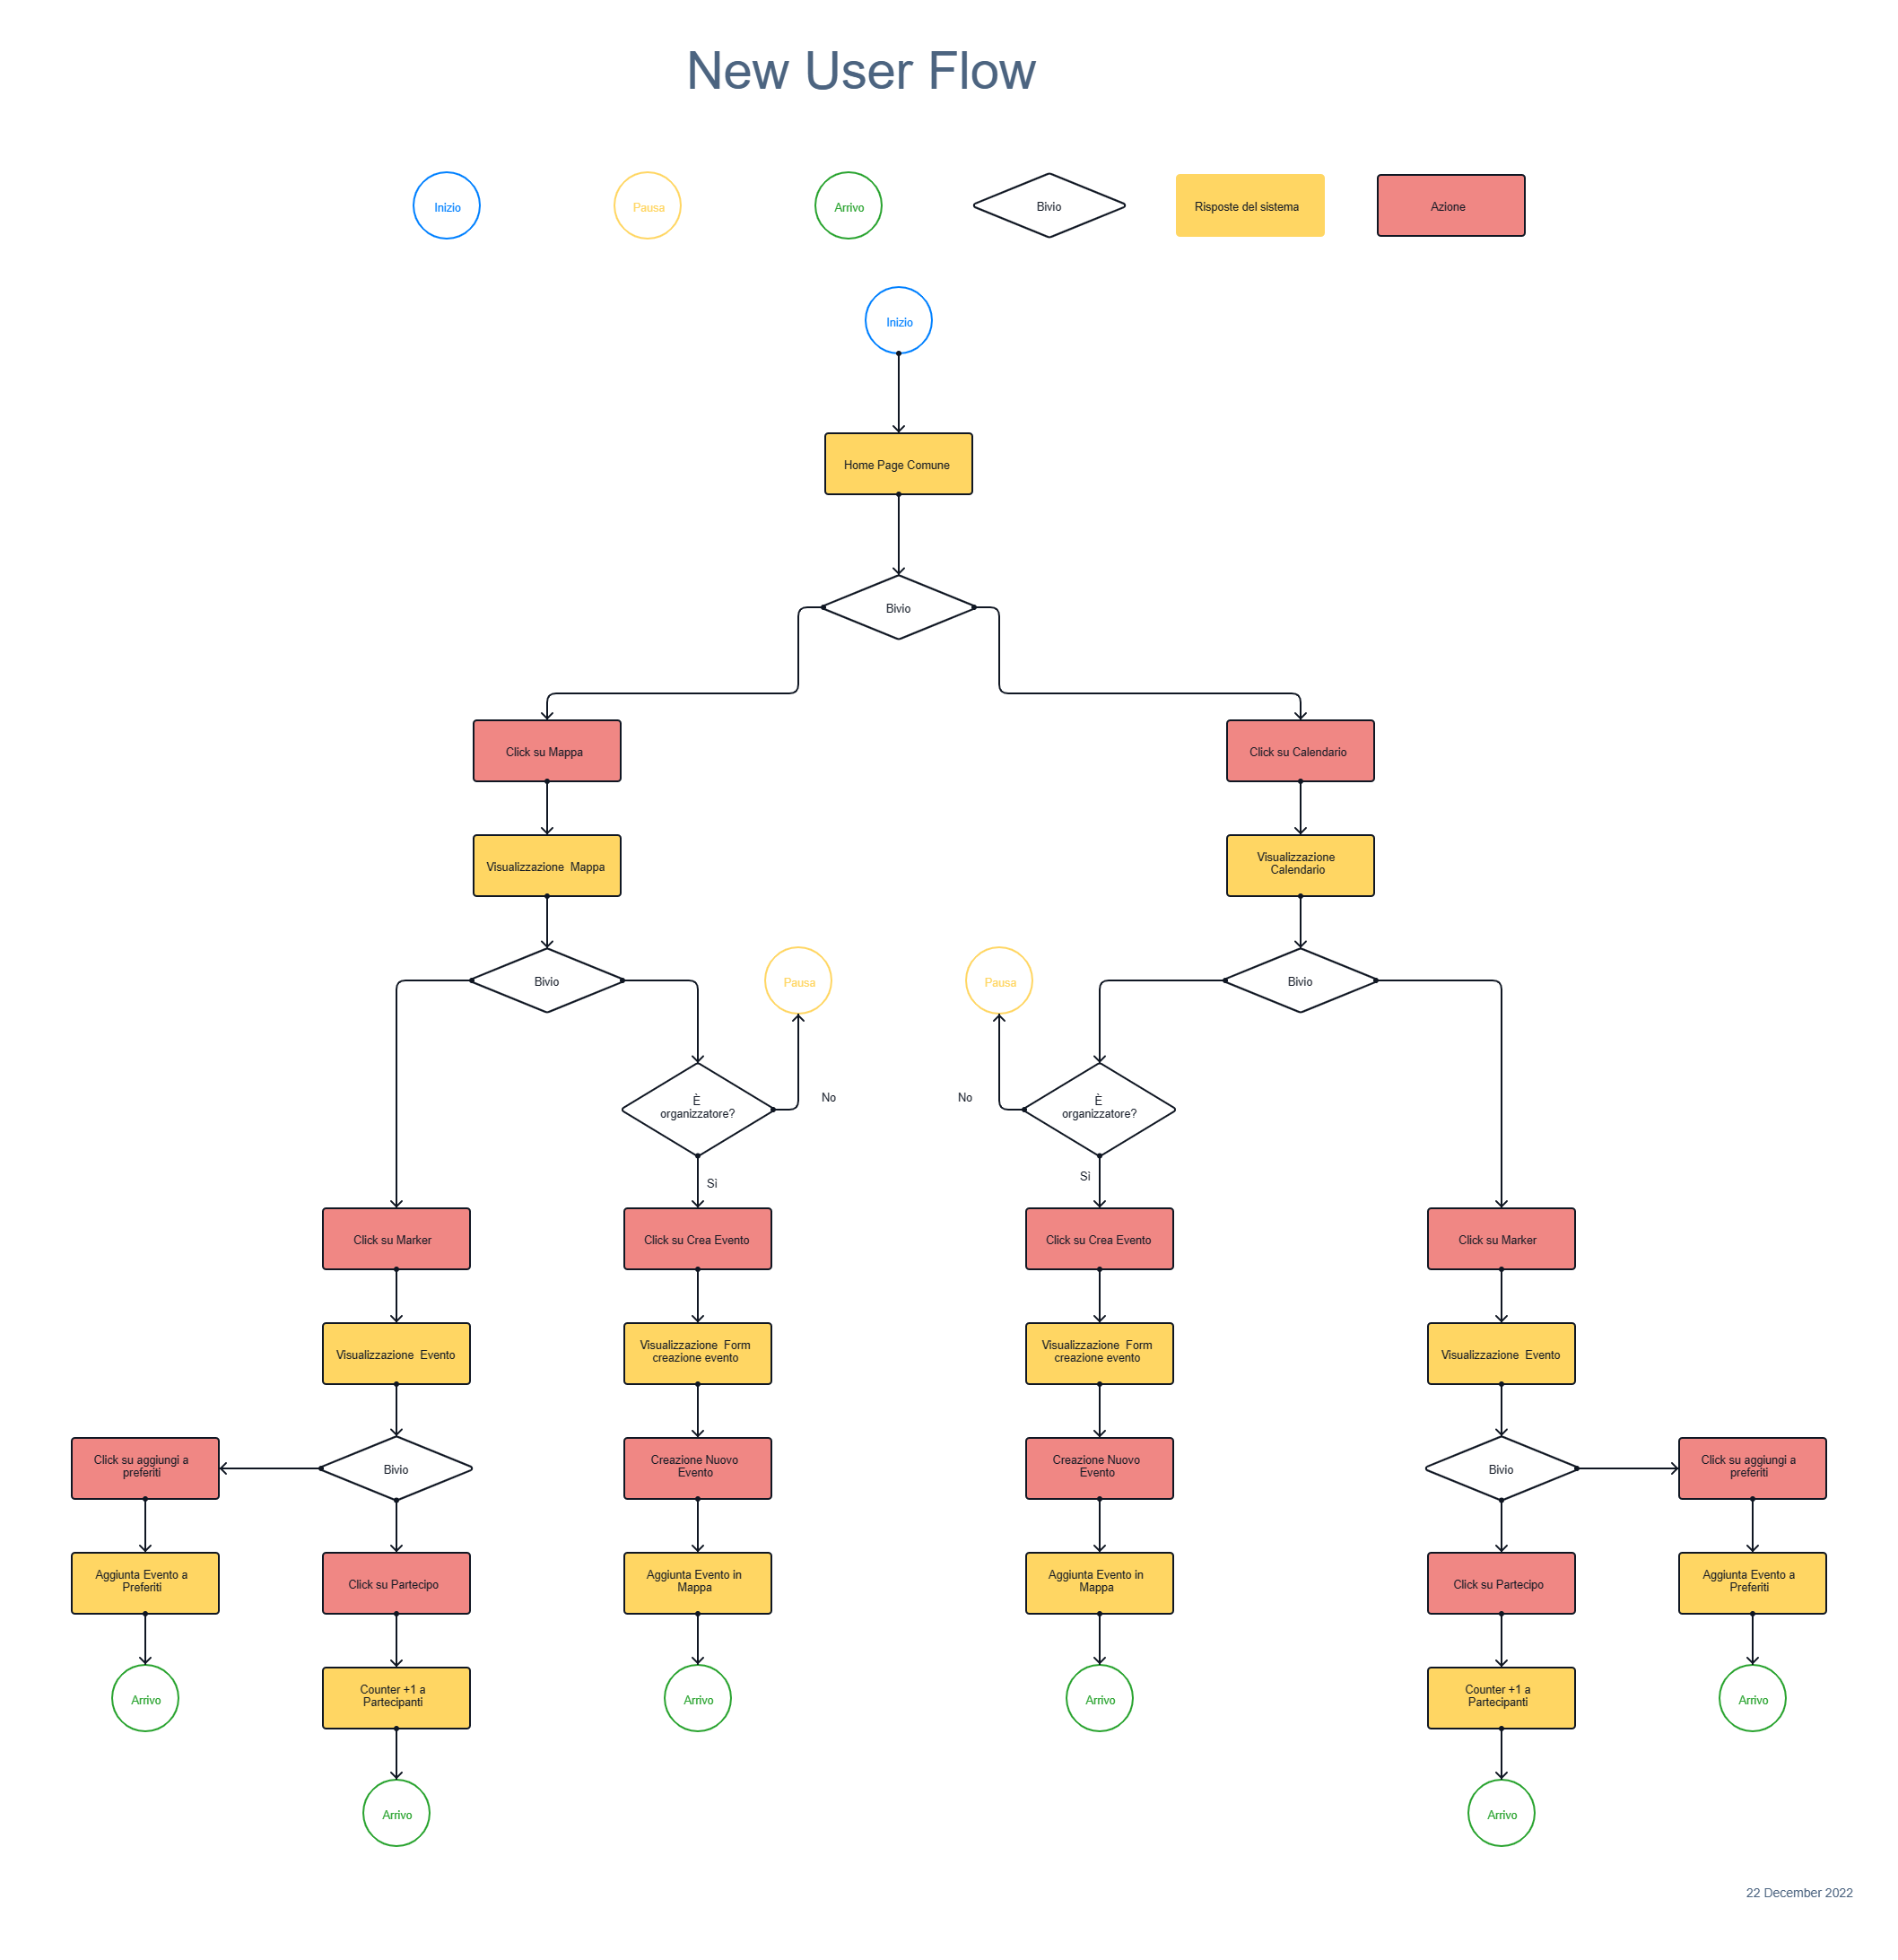
\includegraphics[scale=0.225]{User-Flow.png}
        \end{center}
\end{description}
\clearpage
\section{Application Implementation and Documentation}
\begin{description}
    \item[] Nei precedenti documenti sono stati identificati tutti i requisiti funzionali e non funzionali
        dell'applicazione. Nella sezione precedente son state descritte le features che servono ad un Utente nel
        suo flusso applicativo.
    \item[] Nella seguente sezione vengono analizzati i software e i tools di sviluppo di Fen Festa. L'applicazione è
        stata sviluppata utilizzando React (front-end) e NodeJS (back-end). Per la gestione dei dati è stato
        utilizzato MongoDB.
\end{description}
\end{document}